Introduce the big idea and what we got.

\subsection{Parameter Tuning}

\begin{itemize}
\item 4000 Hz doesn't work! (Burst Plot)

\begin{figure}
\centering
\begin{subfigure}[b]{0.49\textwidth}
\includegraphics[width=\textwidth]{Burst_plot_4000Hz.eps}
\caption{4000 Hz}
\label{burstSTDP:4000}
\end{subfigure}
\,
\begin{subfigure}[b]{0.49\textwidth}
\includegraphics[width=\textwidth]{Burst_plot_6000Hz.eps}
\caption{6000 Hz}
\label{burstSTDP:6000}
\end{subfigure}
\caption{Compare the two}
\label{burstSTDP}
\end{figure}

\item Mention annealing and our choice of \(r_{in}, \eta\) and \(\epsilon\). Name the two data sets we refer to for the remainder of the paper. (Scatter Error Function)

\item Setting \(w_{max}\). (Burst History)
\end{itemize}

\subsection{Convergence and Stability}

\begin{itemize}
\item Demonstrate the stability of our IB model by showing the firing rate plot and how it splits according to \(r_{in}\).

\begin{figure}[H]
\centering
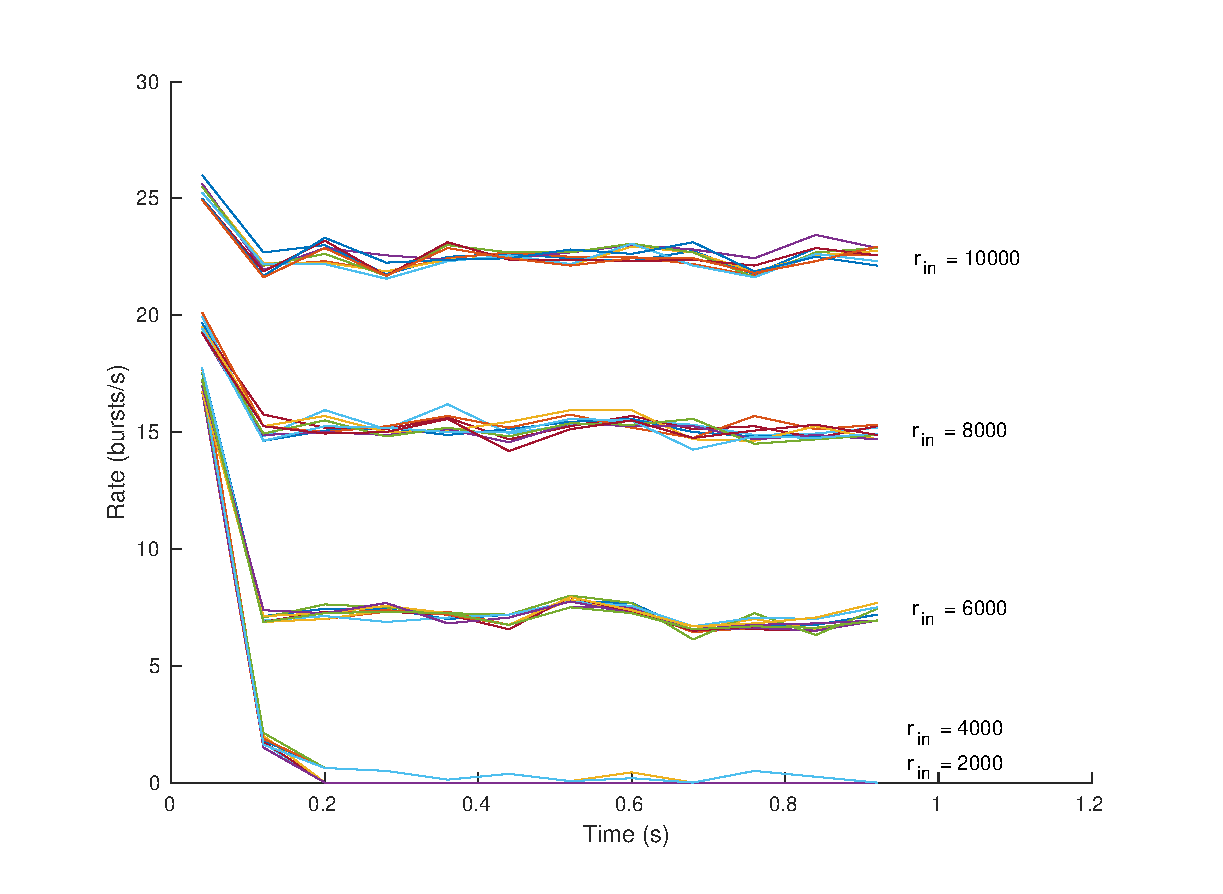
\includegraphics[scale = 0.4]{Firing_Rate_Binsize_80ms.eps}
\label{FR}
\caption{Caption will go here}
\end{figure}

\item Plot Weight and \(WW^T\) for 4000 and 6000 Hz to show some level of convergence.

\item Plot error function over time from normal and from permutation matrix

\item Describe why the error function converges away from 0.
\end{itemize}

\subsection{Hebbian Learning versus STDP}

\begin{itemize}
\item Introduce the idea of the refutation. 
\item Give a theoretical description why the type of learning should be relatively unimportant.
\item Compare plots (\(WW^T\), Error vs Time, Burst History).
\end{itemize}